\documentclass[12pt]{article}

% TEMPLATE DEFAULT PACKAGES
\usepackage{amssymb,amsmath,amsfonts,eurosym,geometry,ulem,graphicx,color,setspace,sectsty,comment,natbib,pdflscape,array,adjustbox}

% ADDED PACKAGES FOR THIS MANUSCRIPT
\usepackage{palatino,newtxmath,multirow,titlesec,threeparttable,tabu,booktabs,titlesec,threeparttable,mathtools,bm,bbm,subcaption,pdflscape,tcolorbox,mathrsfs,tikz,graphicx}
% endfloat,

\usepackage{afterpage}
\usepackage[hyphens]{url}
\usepackage[margin=1cm]{caption}

\usepackage[draft]{hyperref}
\newcommand{\tim}{$\,\times\,$}
% FIGURES & TABLES CAPTION STYLING
\captionsetup[figure]{labelfont={bf},name={Figure},labelsep=period}
\captionsetup[table]{labelfont={bf},name={Table},labelsep=period}

% SECTION TITLE SETTINGS
\titlelabel{\thetitle.\enskip}
\titleformat*{\section}{\large\bfseries}
\titleformat*{\subsection}{\normalsize\bfseries}

% COLUMN TYPES
\newcolumntype{L}[1]{>{\raggedright\let\newline\\\arraybackslash\hspace{0pt}}m{#1}}
\newcolumntype{C}{>{\centering\arraybackslash}p{5.2em}}
\newcolumntype{D}{>{\centering\arraybackslash}p{5em}}
\newcolumntype{R}[1]{>{\raggedleft\let\newline\\\arraybackslash\hspace{0pt}}m{#1}}


% MARGINS AND SPACING
\normalem
\geometry{left=1.1in,right=1.1in,top=1.0in,bottom=1.0in}
\setlength{\parskip}{2.5pt}

% SPECIAL CELL 
\newcommand{\specialcell}[2][c]{%
	\begin{tabular}[#1]{@{}l@{}}#2\end{tabular}}

% NO INDENT ON FOOTNOTES
\usepackage[hang,flushmargin]{footmisc}

\begin{document}

\section*{County-level data}
\begin{itemize}
\item There are around 3,200 counties and 1,000 weather stations (with data from the 1980s)
\item I take nearest weather station to the centroid of each county (could do pop-weighted centroid in the future) (in cases where stations have missing data, I fill in  with the average of the 5 closest stations)
\item makes over 10 million obs.  (3,200 counties for 365 days for 9 years (1980-1988))
\end{itemize}

\section*{Types of variation to leverage}
\begin{enumerate}
\item \textbf{Pre/post policies started} : 25 state disconnection policies launched on or before 1980, and 5 per year in 1981, 1982, and 1983
\item \textbf{Pre/post seasonal implementation} : 31 states have seasonal info (which include 5 distinct start dates and 7 distinct end dates) 
\item \textbf{Temperature Cutoff} : 11 states have broad ``winter'' policies (preventing disconnection during cold weather) and 6 states list specific temperatures (5 are 32 degrees, 1 is 20 degrees) (a couple have summer thresholds but haven't looked there yet)
\end{enumerate}

\section*{Death outcomes}
\begin{enumerate}
\item Three age groups (ages 1-4, ages 5-74, over 75)
\item Two cause categories : (1) Cold-sensitive diseases (septicimia, pneumonia, heart issues, cerebrovascular, TB (based coarsely on Jayachandran's analysis)) and (2) all other causes 
\end{enumerate}

\section*{Two example figures (with different outcomes to see the possibilities)}

\begin{figure}
\centering
\caption{Average Demeaned Deaths (from all causes) By Temp. Before and After Winter policy goes into effect each year}
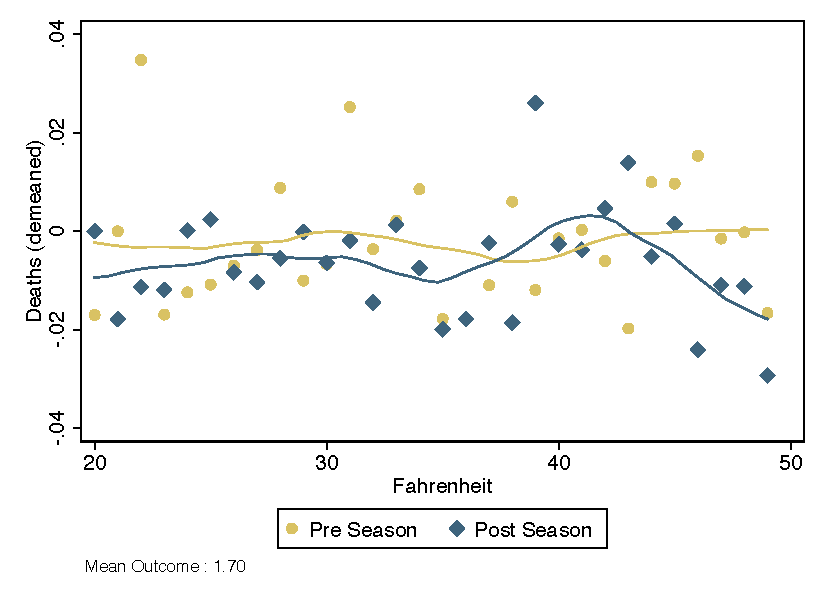
\includegraphics{figures/tgrad_deaths_all.pdf} \\
\begin{itemize}
\item Pre includes 30 days before the winter policy starts and post includes 30 days after the winter policy starts.
\item Deaths include all causes and ages, at the county level.  Deaths are demeaned for (1) calendar day, (2) county-month, (3) county-year.
\item This graph looks pretty good because mortality declines for temperatures below 32 degrees after the policy takes effect; however, the mortality data bounces around a lot and its hard for me to establish if effects are really there.
\item Eyeballing an effect size of around 0.01 deaths seems reasonable because (1) its about 0.005\% of the mean, which is probably consistent with the tiny effects we would expect, and (2) the fixed effects seem to take out enough noise that we might actually be able to identify effects sizes this small
\end{itemize}
\end{figure}



\begin{figure}
\centering
\caption{Average Demeaned Deaths for over 74 yr olds, below 32 degrees, and from cold-sensitive causes by days Before and After Winter policy goes into effect each year}
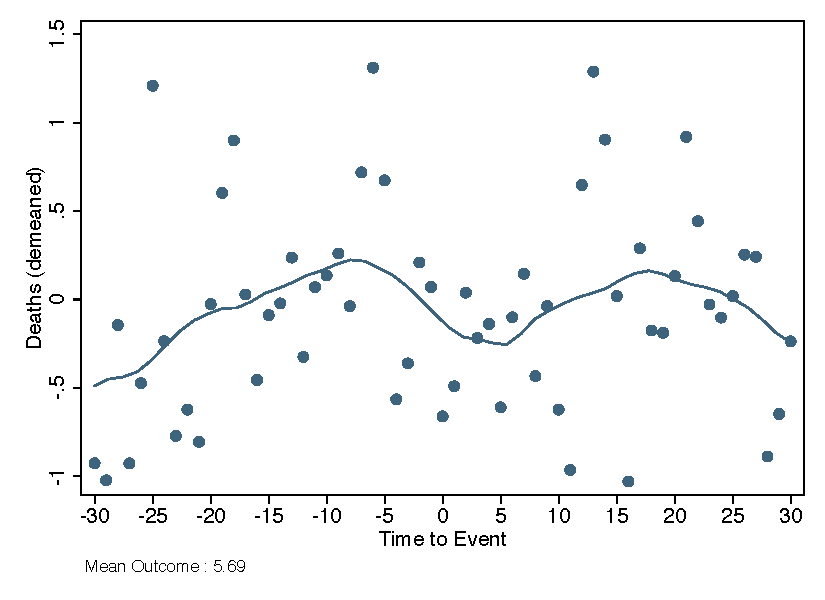
\includegraphics{figures/te_deaths_old_ewm_cold.pdf} \\
\begin{itemize}
%\item Pre includes 30 days before the winter policy starts and post includes 30 days after the winter policy starts.
\item Deaths for people over 74, on days below 32 degrees, from cold-sensitive causes, at the state level.  Deaths are demeaned for (1) calendar day, (2) state-month, (3) state-year.
\item This graph sort of looks good because deaths kind of drop around the time that the policy comes into effect, although its pretty darn noisy
\end{itemize}
\end{figure}









% \begin{itemize}
% \item Plot event-studies before and after seasonal start and end dates (before and after policies are in place)
%     \begin{itemize}
%         \item conduct at state-level (look at cold and warm deaths separately)
%         \item demean by calendar-day and state-year
%     \end{itemize}
% \end{itemize}



\end{document}


